\documentclass[a4paper,10pt]{article}
\usepackage[utf8]{inputenc}
\usepackage[T1]{fontenc}
\usepackage[english,italian]{babel}
\usepackage[hmargin=2cm,vmargin=2cm, bottom=2cm]{geometry}
\usepackage{fancyhdr}%
\usepackage{amsfonts}
\usepackage{graphicx}
\usepackage[ruled]{algorithm2e}
\usepackage{titling}

\setlength{\droptitle}{-5em}   % This is your set screw
\pagestyle{fancy}% Change page style to fancy
\fancyhf{}% Clear header/footer
\fancyhead[C]{Michele Lazzeri | 822879}
\fancyfoot[C]{\thepage}% \fancyfoot[R]{\thepage}
\renewcommand{\headrulewidth}{0.4pt}% Default \headrulewidth is 0.4pt
\renewcommand{\footrulewidth}{0.4pt}% Default \footrulewidth is 0pt
\setlength{\parindent}{0pt}
%inizio custom commands
\newcommand{\grass}[1]{\textbf{#1}}
%fine custom commands

\begin{document}
\author{Michele Lazzeri Matricola 822879}
\title{Progetto di Algoritmi e Strutture Dati}
\date{}
\maketitle
\section{Traduzione da Linguaggio di contesto a Linguaggio specifico}
I 'nucleotidi' {A,T,C,G} rappresentano un Alfabeto $\Sigma$. Una concatenazione di simboli dell'Alfabeto rappresenta una Stringa fr e nel contesto viene chiamato 'Frammento di DNA'. L'insieme di tutti i 'Frammenti di DNA' ammissibili {\large F} rappresenta quindi il Linguaggio.

Un 'enzima' rappresenta una funzione $\epsilon\colon F\to F$. L''insieme degli enzimi' $\varepsilon$ rappresenta quindi una classe di funzioni di questo tipo.

Una 'trasformazione' rappresenta il risultato di un prodotto di funzioni.

Un 'esperimento' rappresenta un insieme di stringhe fr e di enzimi $\epsilon$.

La 'durata' $\Delta$ rappresenta il numero massimo di funzioni applicabili per ogni Stringa fr in ogni esperimento.

L''energia richiesta in UEA' rappresenta una funzione peso che associa ad ogni 'enzima' $\varepsilon$ un numero reale: $energia(\varepsilon)\colon\epsilon\to\mathbb{R_+}$
\\Inoltre $\forall$ trasformazione t $=\{e_1,e_2,\dots,e_k\}$ abbiamo che $energia(t)=\sum_{j=1}^k energia(e_j)$

\section{Scelta delle strutture adatte}
\subsection{Frammenti di Dna / Stringhe}\label{sec:fram}
Il metodo più semplice per immagazzinare le singole stringhe è quello di utilizzare degli array. Gli array:
\begin{itemize}
\item permettono un accesso diretto ad ogni singolo elemento (simbolo);
\item richiedono uno spazio di memoria contenuto
\item sono semplici da gestire e si adattano bene ad operazioni su stringhe. 
\end{itemize}
Una possibile struttura in C potrebbe essere composta in questo modo:
\begin{verbatim}
struct stringa {
    nome char[50];
    int lunghezza;
}
\end{verbatim} In questo modo è possibile inserire nuovi elementi alla fine dell'array senza dovere riallocare l'intera array (supponendo di non superare il limite dei 50 caratteri) in tempo O(1), il rovesciamento dell'array può essere effettuato tramite un array di appoggio in tempo O(n), l'eliminazione degli ultimi n elementi in un tempo O(1), l'eliminazione e l'inserimento di un elemento non alla fine dell'array possono comunque essere realizzati shiftando i vari elementi dell'array. La semplicità della struttura permette in ogni caso di implementare le varie funzioni (gli 'enzimi') facilmente.

\subsection{Libreria degli enzimi}
La libreria degli enzimi raccoglie le varie funzioni disponibili per la manipolazione dei frammenti di DNA.
Le due funzioni che devono essere servite da tale libreria sono char *enzima (char *nome\_{}enzima, char *frammento\_{}src ) e int energia\_{}enzima (char *nome\_{}enzima ).
Tali funzioni possono essere implementate tramite un costrutto \begin{verbatim}
    switch(nome_enzima) {
        case A:
        ...
        case B:
        ...
    }
\end{verbatim} oppure utilizzando un albero binario di ricerca. Quest'ultima opzione garantisce i seguenti benefici:
\begin{itemize}
\item Tempo di accesso proporzionale alla lunghezza dell'albero: tale tempo nel caso peggiore si rivela essere ugualmente $O(n)$, ma nel caso medio il tempo scende a $O(log(n))$, dove n è il numero di enzimi presenti.
\item Tempo di inserimento in qualsiasi posizione: $O(n)$ nel caso peggiore, $O(log(n))$ nel caso medio
\end{itemize} I singoli nodi possono essere strutture formate da un puntatore a funzione, una stringa identificativa e un intero per l'energia richiesta. Tale libreria fornisce le funzioni char *enzima(char *nome-enzima, char *frammento) e int energia-enzima(char *nome-enzima).
Per ridurre il tempo a $O(log(n))$ anche nel caso peggiore si potrebbe ricorrere a una struttura come un albero 2-3 o un B-albero, per semplicità verrà però usato un albero di ricerca binario.
\subsection{Esperimento}
L'intero esperimento può essere rappresentato tramite un grafo ordinato $G=<V,E>$ dove V sono i nodi (in questo caso le varie Stringhe / Frammenti di DNA) e E è un sottoinsieme del prodotto cartesiano $V\times V$ tale che $e = \{x,y\} \in E \iff \exists$ enzima $enz \mid enzima(enz,x)=y$
Convenzioni utilizzate: \begin{itemize}
\item L'energia necessaria per ogni enzima è rappresentata dal peso del lato. \item La possibilità che ad un frammento non si attacchi nessun enzima viene 'emulata' tramite un enzima nullo che restituisce lo stesso frammento. All'interno del grafo tale lato viene raffigurato tramite un cappio.

\end{itemize}
Ad esempio il grafo: \begin{figure}[htop]
\centering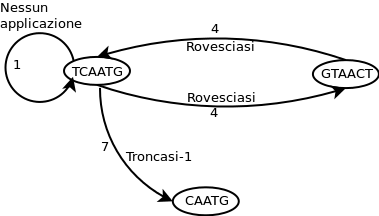
\includegraphics[scale=0.5]{graph1.png}\end{figure}

Rappresenta la situazione per cui:
\begin{itemize}\item 'TCAATG' può diventare 'GTAACT' tramite l'enzima Rovesciasi di peso 4(che 'rovescia' i frammenti) \item 'TCAATG' può diventare 'CAATG' tramite l'enzima troncasi-1 di peso 7
\item 'GTAACT' può diventare 'TCAATG' tramite l'enzima rovesciasi di peso 4
\item 'TCAATG' resta 'TCAATG' senza applicazione di enzimi
\item \dots
\end{itemize}
Il tempo determina il numero di lati e di frammenti, infatti partendo dai frammenti \{'TCA','CTA'\} e dall'enzima Insertasi-1C i grafi al tempo 1 e al tempo 2 sono i seguenti:
\begin{figure}[htop]
\centering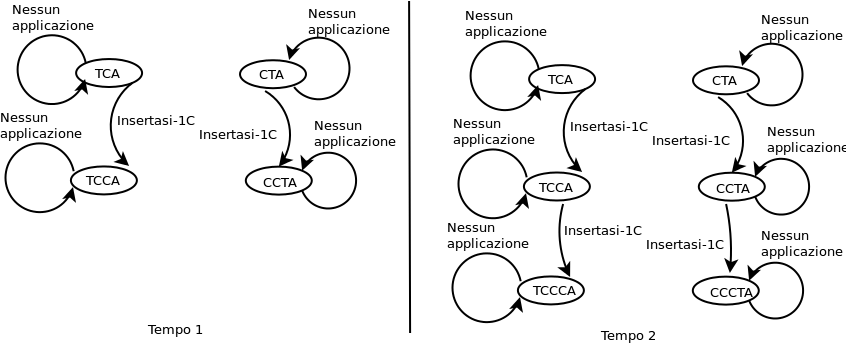
\includegraphics[scale=0.5]{graph2.png}\end{figure}


L'implementazione del grafo avviene tramite liste di adiacenza, con una variazione nella struttura usata per rappresentare i nodi, come spiegato nella sezione \ref{sec:nodi}.

\subsubsection{Inibizione enzimi}
L'inibizione degli enzimi può essere implementata tramite un altro albero di ricerca binaria. Prima dell'avvio dell'esperimento, infatti, la situazione del grafo G è quella di avere un certo numero n di vertici e nessun lato. L'esperimento vero e proprio applica ad ogni vertice tutti gli enzimi contenuti in una struttura che deve essere riempita tramite le chiamate di aggiungi\_enzima. Invece di utilizzare una lista per tale struttura risulta comodo utilizzare un albero di ricerca binaria. Tale albero sarà formato da nodi che conterranno sia il nome dell'enzima, sia un valore booleano che rappresenta se l'enzima è attivo o inibito. In questo modo l'inibizione di un enzima avviene cercando all'interno di tale albero l'enzima e portando a false il valore booleano associato. L'utilizzo di un albero di ricerca binaria invece di una lista permette di velocizzare sia il processo di inibizione/riattivazione sia quello di inserimento.

All'interno dei nodi di quest'albero sarebbe inoltre possibile inserire anche l'energia richiesta per l'attivazione di tale enzima: in questo modo, pur utilizzando una quantità maggiore di spazio (i dati relativi all'energia richiesta sono già disponibili nella libreria degli enzimi) rende più veloce l'accesso a tali informazioni. Infatti se n è il numero di enzimi a disposizione del professore e k è il numero di enzimi utilizzati in questo esperimento abbiamo che $1\le k \le n$.

\subsubsection{I nodi del grafo}\label{sec:nodi}
L'algoritmo per la costruzione del grafo, dopo l'inserimento dei frammenti iniziali e degli enzimi ha una struttura generale del tipo

\begin{algorithm}[H]
\For{nodo v $\in$ V}{
\For{enzima $\epsilon\in\varepsilon$}{
z:= enzima($\epsilon$,v)\;
a:= cerca(z)\;
\uIf{$\exists$ z in V}{k:= puntatore al nodo preesistente che contiene z}
\Else{crea nodo(z)\;
k:= puntatore a tale nodo\;
}
L(v) := INSERISCI(($\epsilon$,k))\;
}}
\end{algorithm}
Dove $\varepsilon$ è l'insieme degli enzimi inseriti nell'esperimento, V è l'insieme dei nodi, L(v) è la lista di adiacenza del nodo v.

Data la necessità, dopo l'ottenimento del risultato della funzione enzima($\epsilon$,stringa), di cercare se tale risultato è già presente nella lista dei nodi (in modo tale da creare un lato dalla stringa di origine al risultato) risulta comodo utilizzare anche per la lista dei nodi un albero binario di ricerca, per ridurre tali tempi di ricerca.

L'implementazione scelta per la creazione del grafo risulta quindi essere formata da una struttura (che verrà chiamata Struct) contenente due puntatori, uno all'albero contenente i frammenti (il grafo orientato vero e proprio)(Albero\_{}Framm) e un altro verso l'albero contenente gli enzimi inseriti nell'esperimento (Albero\_{}Enz)
\begin{itemize}
\item l'albero contenente i frammenti avrà dei nodi formati da 5 campi: 
\begin{itemize}
\item Il frammento di DNA, implementato come descritto in \ref{sec:fram};
\item Due puntatori, uno al figlio sinistro e uno al figlio destro
\item Un puntatore alla lista di adiacenza (ogni elemento di tale lista sarà formata da un campo nome, che conterrà il nome dell'enzima, e un puntatore al frammento risultante dall'applicazione dell'enzima sul frammento originario)
\item Un valore che indica se tale nodo è stato visitato o meno (spiegazione in \ref{sec:esp})
\end{itemize}
\item l'albero contenente gli enzimi inseriti avrà dei nodi formati da 4 campi:
\begin{itemize}
\item Il nome dell'enzima
\item Due puntatori, uno al figlio sinistro e uno al figlio destro
\item Un valore booleano che indica se tale enzima è attivo o meno
\end{itemize}
\end{itemize}
Anche per questi due alberi per ridurre il tempo di inserimento/ricerca/cancellazione a $O(log(n))$ anche nel caso peggiore si potrebbe ricorrere a una struttura come un albero 2-3 o un B-albero, ma per semplicità verrà usato un albero di ricerca binario.

\section{Funzioni in pseudo-codice}
\subsection{Crea\_{}Nuovo}
Questa prima funzione crea semplicemente la struttura di base e inserisce nell'albero degli enzimi l'enzima nullo (di peso 1) rappresentante la non-interazione tra enzimi e frammenti:

\begin{algorithm}[H]
A:= Albero Binario\;
B:= Albero Binario\;
B:= INSERISCI(B,('Nessuna Trasformazione',1))\;
Struct:= INSERISCI(Struct,(A,B))\;
return Struct\;
\end{algorithm}
La procedura richiede un tempo O(1) dovendo semplicemente allocare spazio e inserire al primo posto di un albero senza vertici un nodo.
\subsection{Cerca(el,rad)}
Questa funzione cerca un nodo el all'interno di un albero binario di ricerca con radice rad, se lo trova restituisce la coppia (1,\&{}nodo), se non lo trova restituisce la coppia (0,\&{}padre). In questo secondo caso l'inserimento non richiederà più di trovare il cammino fino ad una foglia, ma basterà confrontare l'elemento da inserire con padre e inserire quindi l'elemento come figlio destro o sinistro:

\begin{algorithm}[H]
node:= rad\;
\uIf {rad = el}{return 1,node\;}
\uElseIf {rad < el}{
\eIf {des(rad) $\neq$ NULL}{return cerca(el,des(rad))}{return 0,node\;}}
\ElseIf {rad > frammento}{
\eIf {sin(rad) $\neq$ NULL}{return cerca(el,sin(rad))}{return 0,node\;}}
\end{algorithm}
Tale procedura ricorsiva effettua un numero di chiamate proporzionale all'altezza dell'albero. Se l'albero è bilanciato l'altezza è dell'ordine di log(n) dove n è il numero dei nodi, se non lo è l'ordine è quello di n. La procedura richiede quindi un tempo $O(log(n))$ nel caso medio e $O(n)$ nel caso peggiore.
\subsection{Nuovo\_{}Frammento(frammento)}
Questa procedura chiama inizialmente la procedura cerca, se cerca ritorna 1 allora la procedura si arresta, se ritorna 0 confronta il nodo ritornato da cerca con frammento e inserisce quest'ultimo come figlio sinistro o destro:

\begin{algorithm}[H]
(a,padre) := cerca(frammento,radice(Albero\_{}Framm))\;
\If {a=0}{
\eIf{padre > frammento}{sin(padre):= frammento}{des(padre):= frammento}
}
\end{algorithm}
Il costo dell'inserimento risulta quindi tutto attribuito alla procedura cerca ed è quindi nuovamente dell'ordine di $O(n)$ nel caso peggiore e $O(log(n))$ nel caso medio.
\subsection{Nuovo\_{}Frammento\_{}vis(frammento)}
Questa funzione, molto simile alla precedente, inserisce un frammento, ma con la differenza che nel caso in cui venga inserito un nuovo frammento imposta il campo visitato a 1 e restituisce un puntatore al nodo creato.

\begin{algorithm}[H]
(a,node) := cerca(frammento,radice(Albero\_{}Framm))\;
\If {a=0}{
\eIf{padre > frammento}{sin(node):= (frammento,1)\;
node:= sin(node)\;}{des(node):= (frammento,1)\;node:= des(node)}

}return node\;
\end{algorithm}
\subsection{Nuovo\_{}Enzima(enzima)}
Questa funzione cerca l'enzima all'interno del corrispettivo albero, se lo trova lo attiva, se non lo trova crea un nuovo nodo con il flag attivato

\begin{algorithm}[H]
(a,padre) := cerca(enzima,radice(Albero\_{}Enz))\;
\eIf {a=0}{
\eIf{padre > enzima}{sin(padre):= (enzima,1)}{des(padre):= (enzima,1)}
}{padre.attivato:= 1}
\end{algorithm}
\subsection{Cancella\_{}enz(nodo)}
Questa funzione elimina l'albero degli enzimi partendo dalla radice nodo

\begin{algorithm}[H]
\If{sin(nodo) $\neq$ NULL}{cancella\_{}enz(sin(nodo))}
\If{des(nodo) $\neq$ NULL}{cancella\_{}enz(des(nodo))}
cancella nodo;
\end{algorithm}
Il numero delle chiamate è proporzionale al numero degli enzimi.
\subsection{Cancella\_{}framm(nodo)}
Questa funzione elimina l'albero dei frammenti partendo dalla radice nodo

\begin{algorithm}[H]
\If{sin(nodo) $\neq$ NULL}{cancella\_{}enz(sin(nodo))}
\If{des(nodo) $\neq$ NULL}{cancella\_{}enz(des(nodo))}
\For{e $\in$ L(nodo)}{cancella e}
cancella nodo;
\end{algorithm}
Le chiamate sono proporzionali al numero totale di archi (per la cancellazione delle liste di adiacenza) e al numero di frammenti.
\subsection{Elimina\_{}Enzima(enzima)}
Questa funzione cerca nell'albero degli enzimi se è presente l'enzima e se lo è lo inibisce:

\begin{algorithm}[H]
(a,enzima):= cerca(enzima)\;
\If{a=1}{enzima.attivo:= 0}
\end{algorithm}
Anche per questo algoritmo la ricerca è la componente che determina il costo in tempo
\subsection{Prepara\_{}Esperimento(f\_{}file, e\_{}file)}
Questa funzione ricrea la struttura di base e inserisce nei due alberi i frammenti e gli enzimi presi rispettivamente dai file f\_{}file e e\_{}file:

\begin{algorithm}[H]
\If {struct esiste}{cancella\_{}enz()\;
cancella\_{}framm()\;
cancella struct\;}
nuovo\_{}esperimento()\;
\For {f in f\_{}file}{nuovo\_{}Frammento(f)}
\For {e in e\_{}file}{nuovo\_{}Enzima(e)}


\end{algorithm}
\subsection{esp(tempo)}\label{sec:esp}
Questa funzione fa agire gli enzimi su ogni frammento e confronta i risultati con i frammenti già presenti, inserisce i nuovi frammenti e crea nelle liste di adiacenza i puntatori per i vari nodi adiacenti:

\begin{algorithm}[H]
\If{tempo > 0}{
\For{t=1,2\dots{}tempo}{
\For{f $\in$ Albero\_{}frammenti}{
\If{f.visitato:= 1}{
f.visitato:=0\;
}
}
\For{f $\in$ Albero\_{}frammenti}{
\If{f.visitato=0}{
\For{e $\in$ Albero\_{}enzimi}{
\If{e.attivato=1}{
z:= enzima(e,f)\;
k:= nuovo\_{}Frammento\_{}vis(z)\;
L(f):= INSERISCI(L(f),(en,k))\;
}}
f.visitato:= 2\;
}
}
}
}
\end{algorithm}
Come si può notare, dato che l'inserimento di un nuovo frammento è all'interno di un ciclo for che scansiona tutti gli elementi dell'albero dei frammenti, se il frammento fosse inserito senza utilizzare il flag visitato la funzione andrebbe in Loop: supponendo ad esempio di avere il solo frammento 'TAC' e l'enzima 'Insertasi-1A' la procedura inserirebbe 'TAAC', il ciclo for prenderebbe 'TAAC' come altro frammento e ad esso applicherebbe nuovamente l'enzima e così via. Creando invece il campo visitato, i frammenti vengono impostati inizialmente a 0 e ogni frammento inserito avrà il flag visitato impostato a 1, non verrà quindi riselezionato dal ciclo for. Inoltre gli elementi a cui sono stati applicati gli enzimi al tempo n non andranno riconsiderati al tempo n+1 e il campo visitato assume il valore 2. 2 significa quindi che il frammento è già stato utilizzato nell'esperimento, 1 che sarà utilizzato nel prossimo 'tempo' e 0 che deve essere utilizzato durante questo 'tempo'.

Questa procedura è una delle più dispendiose in termini di tempo dell'intero progetto, infatti supponendo che gli enzimi creino sempre frammenti non esistenti:

indicando con $|F|$ il numero dei frammenti iniziali e con $|E|$ il numero degli enzimi attivati la procedura richiede:
\begin{itemize}
\item al \grass{primo} passo il ciclo for dei frammenti cicla $|F|$ volte e quello interno degli enzimi $|E|$ volte, quindi Nuovo\_{}Frammento\_{}vis viene chiamato $|F|*|E|$ volte
\item al \grass{secondo} passo il ciclo for dei frammenti cicla $|F|*|E|$ volte e quello interno degli enzimi $|E|$ volte, quindi Nuovo\_{}Frammento\_{}vis viene chiamato $|F|*|E|*|E|$ volte
\item \dots
\item al \grass{n-esimo} passo il ciclo for dei frammenti cicla $|F|*|E|^{n-1}$ volte e quello interno degli enzimi |E| volte, quindi Nuovo\_{}Frammento\_{}vis viene chiamato $|F|*|E|^n$ volte
\end{itemize}
Nel caso medio Nuovo\_{}Frammento\_{}vis richiede un tempo $O(log(n))$ e quindi il tempo totale risulta essere \begin{displaymath}\sum_{n=1}^{tempo}{(f*e^n*O(log(f*e^{n-1}))}
\end{displaymath}
da cui \begin{displaymath}
f*O(log(f))\sum_{n=1}^{tempo}{(e^n)} + f*O(log(e))\sum_{n=1}^{tempo}{((n-1)(e^n))}
\end{displaymath}
e quindi \begin{displaymath}
T(f,e,tempo) = O(f*log(e)*e^{tempo})
\end{displaymath}

\subsection{Esperimento(tempo)}
Questa funzione chiama esp(tempo) e ne stampa i risultati

\begin{algorithm}[H]
\If{tempo > =}{esp(tempo)}
Stampa Albero\_{}Frammenti\;
\end{algorithm}
\newpage\subsection{Dijkstra(V,*funz,s)}
Questa funzione, esempio di Algoritmo greedy, data come istanza un grafo orientato pesato, crea tre vettori: il primo vettore C specifica per ogni nodo v il costo del cammino minimo da f a v, il secondo vettore P specifica il nodo precedente nel cammino da f a v, il terzo vettore N contiene stringhe indicanti il nome dell'ultimo lato nel cammino da f a v. Ad ogni passo viene scelto il lato {u,v} con peso minore e viene inserito nella soluzione a patto che non esista già un cammino con peso minore dalla sorgente a v.

\begin{algorithm}[H]
D:= HEAP\;
D:= INSERT(D,s)\;
\For{v $\in$ V}{C(v):= $\infty$\; P(v):= NULL}
C(s):= 0\;
\While{ISEMPTY(D)=0}{
g:= nodo tale che C(nodo) sia minore\;
D:= DELETE(D,g)\;
\For{u $\in$ L(g) $\land$ C(g)+(*funz)(u.nome\_{}enzima) < 0}{
\If{C(u)=$\infty$}{D:= INSERT(D,u)}
C(u):= C(g)+(*funz)(u.nome\_{}enzima)\;
P(u):= g\;
N(u):= u.nome\_{}enzima\;
}
}
return C,P,N\;
\end{algorithm}
Ricordo che la lista di adiacenza di un vertice è formata da nodi al cui interno è contenuto anche il nome del lato che è il nome dell'enzima.
\subsection{Enzimi(f,g,$\varepsilon$,tempo}
Questa funzione elimina le strutture presenti, ricrea un esperimento, inserisce f come unico frammento, inserisce tutti gli enzimi nell'esperimento, chiama esp(tempo), calcola quindi il cammino minimo da f a g supponendo che gli archi abbiano tutti 1 come peso tramite l'algoritmo di Dijkstra e stampa il risultato

\begin{algorithm}[H]
\If {struct esiste}{cancella\_{}enz()\;
cancella\_{}framm()\;
cancella struct\;}
nuovo\_{}esperimento()\;
nuovo\_{}Frammento(f)\;
\For {e $\in$ $\varepsilon$}{Nuovo\_{}Enzima(e)}
esp(tempo)\;
(C,P,N)=dijkstra(Albero\_{}Framm,*(funzione(Funzione\_{}che\_{}ritorna\_{}1)),f)\;
\eIf{C(g)=$\infty$}{Stampa 'Non ci sono cammini da f a g'}{
S:= STACK\;
\While{P(g) $\neq$ NULL}{
S:= INSERT(S,N(g))\;
g:= P(g)\;
}
STAMPA S\;
}
\end{algorithm}
Il tempo di esecuzione di questa funzione dipende dalle due chiamate esp(tempo) e dijkstra(\dots{}). 
\subsection{Energia(f,g,$\varepsilon '$,tempo)}
Questa funzione fa praticamente la stessa cosa della precedente (cammini minimi) ma passa alla funzione Dijkstra un puntatore alla funzione energia\_{}enzima che restituisce l'ammontare in UEA per ogni enzima.

\begin{algorithm}[H]
\If {struct esiste}{cancella\_{}enz()\;
cancella\_{}framm()\;
cancella struct\;}
nuovo\_{}esperimento()\;
nuovo\_{}Frammento(f)\;
\For {e $\in$ $\varepsilon'$}{Nuovo\_{}Enzima(e)}
esp(tempo)\;
(C,P,N)=dijkstra(rad,*(funzione(energia\_{}enzima)),f)\;
\eIf{C(g)=$\infty$}{Stampa 'Non ci sono cammini da f a g'}{
S:= STACK\;
\While{P(g) $\neq$ NULL}{
S:= INSERT(S,N(g))\;
g:= P(g)\;
}
STAMPA S\;
}
\end{algorithm}
\subsection{Similarità(f,g)}
Questa funzione utilizza la programmazione dinamica per stabilire la similarità di due stringhe. In particolare vengono create due matrici, la prima serve per contenere i valori di similarità delle varie sotto-stringhe, la seconda per ritrovare le coppie formatesi.
Supponendo di avere due stringhe s1,s2 di dimensione N1,N2 le due matrici avranno dimensione N1+1,N2+1. La matrice inizialmente sarà formata da valori del tipo
$M_{j,k}$ = $\left\{\begin{array}{ll}1 & \mbox{se } s1[j-1]=s2[k-1]\\0 & else\end{array}\right.$
Passando poi di cella in cella da sinistra a destra, dall'alto verso il basso viene poi fatto un calcolo sul massimo tra tre valori:
$M_{j,k}$ = max $\left\{\begin{array}{l}M_{j-1,k-1}+M_{j,k}\\M_{j-1,k}\\M_{j,k-1}\end{array}\right.$

In questo modo si sfrutta la programmazione dinamica, in quanto la risoluzione del problema viene suddivisa in sotto-problemi, che vengono utilizza più volte per la costruzione del risultato finale.

\begin{algorithm}[H]
\For{i=0,1...N1}{
M[0][i]:= 0;}
\For{i=0,1...N2}{
M[i][0]:= 0;}
\For{i=1,2...N2}{
\For{j=1,2...N1}{
\eIf{s2[i-1]=s1[j-1]}{a:=M[i-1][j-1]+1;}{a:=M[i-1][j-1]}
b:=M[i-1][j]\;
c:=M[i][j-1]\;
M[i][j]=MASSIMO(a,b,c)\;
\uIf{M[i][j]=a}{T[i][j]='d';}
\uElseIf{M[i][j]=b}{T[i][j]='1';}
\Else{T[i][j]='2';}


}
}

S:= STACK\;
a:= N1\;
b:= N2\;
\While{a>0 $\land$ b>0}{
\uIf{T[a][b]='d'}{a:=a-1\;b:=b-1\;
\If{s1[a]=s2[b]}{S:=INSERISCI(S,s1[a])}}
\uElseIf{T[a][b]='1'}{a:=a-1\;}
\Else{b:=b-1;}
}

Stampa S\;
\end{algorithm}
Tempo e spazio sono entrambi dell'ordine di grandezza di $O(n*m)$ dove n e m rappresentano la lunghezza delle due stringhe.

\end{document}
